\documentclass[]{article}
\usepackage[utf8]{inputenc}
\usepackage{graphicx}
\usepackage{float}
\usepackage[T1]{fontenc}
\usepackage{cite}

\usepackage{url}
\usepackage[portuguese]{babel}
\usepackage[T1]{fontenc}

\newcommand\x[1]{\discretionary{#1}{#1}{#1}}

\graphicspath{ {figs/} }
\title{Predizendo ní­veis de pobreza utilizando imagens de satélites e formulários socioeconômicos}
\author{João Pedro Donaire Albino }
\date{Junho 2019}

\begin{document}


\begin{center}
	\renewcommand{\baselinestretch}{1}
\end{center}

\vspace*{1cm}

\begin{center}
	\textbf{Relatório final de Iniciação Científica}
	
	\vspace*{1cm}
	
	\renewcommand{\baselinestretch}{2}
	\bf {\huge \sc Predizendo níveis de pobreza utilizando imagens de satélites e formulários socieconômicos.}
	\renewcommand{\baselinestretch}{1}
	
\end{center}

\vspace*{2.0cm}

\begin{center}
	
	\large João Pedro Donaire Albino
	
	\vspace*{1.0cm}
	
	\large Orientador:
	\large Prof. Dr. Clayton Pereira
	
	\vspace*{0.5cm}
	
	Departamento de Computação, Faculdade de Ciências, Universidade Estadual Paulista Júlio de Mesquita Filho\\
	Av. Eng. Luiz Edmundo Carrijo Coube, 14-01 - Vargem Limpa, CEP 17033-360 - Bauru - SP.
	
\end{center}

\vspace*{2.0cm}

\centerline{\large \today}

\newpage

\section{Introdução}
\label{s.introducao}

A pobreza é uma das chagas complexas e importantes de nossa sociedade, pois se trata de um problema dificilmente controlado e trabalhado por métodos efetivos de combate ~\cite{ref_pobreza1}. Atrelado a isso também temos uma escassez de dados relevantes que possam mensurar com consistência indicadores de qualidade de vida e de poder aquisitivo da população. Esses dois fatores desencadeiam um notável esforço para mapear e diagnosticar o cenário da pobreza em determinadas regiões, assim perpetuando o problema da má distribuição de renda no país \cite{ref_ma_distribuicao}.

Por outro lado, atualmente, a gestão de dados no Brasil melhorou, porém ainda existe muito o que se desenvolver. No ano de 2018, houve uma iniciativa federal para chamada GovData \cite{ref_govdata}, que fornece uma plataforma para análise e cruzamento de dados. A finalidade principal se dá para que órgãos públicos consigam "melhorar a efetividade e a transparência de políticas públicas sociais implementadas pelo governo". Porém, um serviço muito parecido Open Data \cite{ref_opendata} já em 2007 era utilizado nos EUA, o que mostra o paulatino progresso na análise de dados no Brasil.

\subsection{Origem do Tema}
A necessidade de mapeamento sobre pobreza sempre foi algo necessário e a aplicação de métodos para diminuir custos é algo que pode auxiliar na sua realização. Por tanto, trazer métodos tecnológicos para é algo que poderia auxiliar em tal tema, facilitando a aplicação de recursos financeiros, normalmente governamentais, para problemas que de fato poderiam ser combatidos com investimentos.

\subsection{Justificativa da Pesquisa}
Em setembro de 2015, líderes dos 193 países membros da Organização das Nações Unidas (ONU) aprovaram um plano global de desenvolvimento sustentável, com o objetivo de melhorar os indicadores econômicos, sociais e ambientais para as próximas gerações\cite{ref_nacoes}. Algo relevante para a proposta de pesquisa em questão é averiguar que a primeira dessas metas configura-se em eliminar todas as formas de pobreza no mundo. Essa decisão foi tomada ao levar em consideração que cerca de 705,5 milhões de pessoas vivem atualmente na extrema pobreza \cite{ref_extrema_pobreza}. 

Para exemplificar através de dados locais, uma das principais dificuldades do Brasil reside em direcionar recursos para as população mais pobre \cite{ref_lazarotto}. Mesmo que através de formulários e pesquisas se torna possível identificar regiões com altos índices de pobreza, sofre-se em obter dados relevantes que mensuram, indicam e agrupam regiões por níveis de renda ou outras indicadores importantes.

Outro ponto relevante para se levar em consideração na proposta do trabalho diz respeito à quantidade de investimentos necessários para realizar uma pesquisa intensiva bem esclarecedora sobre indicadores de pobreza. Se levarmos em consideração países que não possuem recursos abundantes, obter dados relevantes se torna algo difícil. Segundo o próprio Instituto Brasileiro de Geografia e Estatística (IBGE), o orçamento do Censo de 2010 realizado no país fora calculado em R\$ 1,677 bilhão \cite{ref_IBGE}.

Analisando tais fatos, chega-se em uma investida para inferir indicadores precisos utilizando dados \textit{open-source}  disponíveis na \textit{Internet}. Esse é um dos tópicos que a Tecnologia de Dados que há algum tempo vem sendo trabalhado e será tratado dentro desta pesquisa.

\subsection{Formulação do problema}
É possível correlacionar intensidade luminosa com riqueza econômica utilizando dados abertos e Machine Learning?

\subsection{Objetivos da Pesquisa}
A pesquisa tinha como escopo principal criar um sistema utilizando Python e R totalmente automatizado para extrair, estruturar, carregar e classificar imagens de satélites noturnos do Estado de São Paulo, sendo estes de origem open-source.

\subsection{Estrutura do Trabalho}
O capítulo 1 discute-se sobre a introdução da pesquisa e objetivos da mesma. Nos dois seguintes trabalha-se apoio teórico e bibliográfico sobre o tema bem como metodologias de pesquisa aplicadas ao mesmo. O capítulo 4 apresenta alguns dados coletados no desenvolvimento da pesquisa e o 5, por sua vez, as considerações finais sobre o desenvolvimento da pesquisa.

\pagebreak


\section{Rerenferencial Teórico}
\label{s.referencia_teorico}
Algo discutido nos últimos tempos é a relação entre intensidade luminosa e pobreza, bem como a presunção de que a mesma pode ou não ser utilizada para correlacionar indicadores de riqueza. Segundo Ebener, et. al, métodos que utilizam informações distribuídas espacialmente, incluindo a luz noturna imagens e população para modelar a distribuição de renda per capita, fornecem resultados promissores para a comparação \cite{ref_ebener}. Bem como provam-se que dados de sensoriamento remoto de luz noturna são possíveis de correlacionar com os números nacionais do Produto Interno Bruto (PIB) dando uma grande relação intensidades luminosas com poder de consumo\cite{ref_mapping_dmsp}.

Importante salientar a definição de PIB. O Produto Interno Bruto faz referência "ao valor agregado, depurado das transações intermediárias e medido a preços de mercado, de todos os bens e serviços finais produzidos dentro do território econômico do país sob consideração\cite{ref_rossetti}.

\subsection{Kmeans}
Basicamente, pode-se mostrar que o algoritmo k-means a cada passo encontra uma melhor solução para o problema de encontrar centros que minimizam o quadrado da distância entre o centro e os dados daquele grupo. Basicamente, algoritmos de clustering têm como função agrupar objetos de dados com base apenas em informações encontradas em dados que descrevem os objetos e suas relacionamentos.

Dado k, o funcionamento básico do algoritmo é resumido em:
\begin{enumerate}
	
	\item Escolha aleatória de k pontos de dados para serem os iniciais;
	
	\item Atribuição de cada ponto de dados ao centróide mais próximo;
	
	\item Recálculo dos centróides usando o cluster atual; E
	
	\item Se um critério de convergência não for cumprido, os passos 2 e 3 são repetidos.
\end{enumerate}

\begin{figure}[!ht]
	\centerline{
		\begin{tabular}{c}
			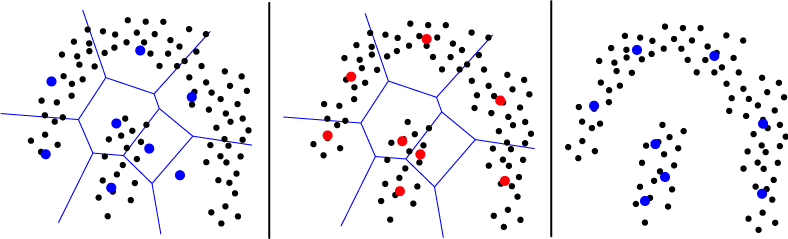
\includegraphics[width=7cm]{figs/kmeans.png}\\
		\end{tabular}
	}
	
	\caption{Funcionamento básico de uma algoritmo Kmeans \cite{ref_kmeans}}		
	\label{f.expl_kmeans}
	
\end{figure}

Segundo Nunes, K-means é um algoritmo que detém um conjunto de dados D = {x} n i=i com n pontos num espaço de dimensão d. Sendo C = {C1, C2, . . . , Ck} um clustering do conjunto de dados. Para cada cluster Ci existe um ponto zi que o representa e que é designado por centróide\cite{ref_nunes}.

\begin{figure}[!ht]
	\centerline{
		\begin{tabular}{c}
			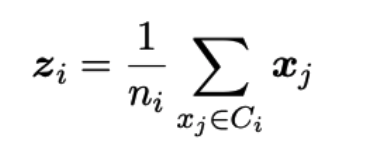
\includegraphics[width=2.4cm]{figs/kmeans-alg.png}\\
		\end{tabular}
	}
	\caption{Fórmula de Kmeans\cite{ref_nunes}}		
	\label{f.nunes}
	
\end{figure}

Segundo o estudo \textit{The k-means clustering technique: General considerations and implementation in Mathematica k-means clustering}, avaliou-se como simples e elegante no modo de particionar conjuntos de dados. Em contrapartida, o K-Means peca em não manipular dados não-globulares de tamanhos e densidades diferentes, além de não identificar outliers\cite{ref_sonagara}.

\subsection{SVM}
O Support Vector Machine, também conhecido como Máquina de Suporte Vetorial é um algoritmo de aprendizado supervisionado, cujo objetivo é classificar determinado conjunto de pontos de dados que são mapeados para um espaço de características multidimensionais usando uma função kernel\cite{ref_svm}.

A visão básico do SVM encontra um hiperplano como a solução para o problema de aprendizagem. A formulação mais simples do SVM é a linear, onde o hiperplano se encontra no espaço dos dados de entrada x. O hiperplano é um subespaço dimensional (n menos 1) para um espaço n-dimensional. Neste caso, o espaço da hipótese é um subconjunto de todas hiperplanos. Além disso, SVMs maximizam a margem em torno do hiperplano de separação, o que fornece algum reforço para que os pontos de dados futuros possam ser classificados com mais confiança.

\begin{figure}[!ht]
	\centerline{
		\begin{tabular}{c}
			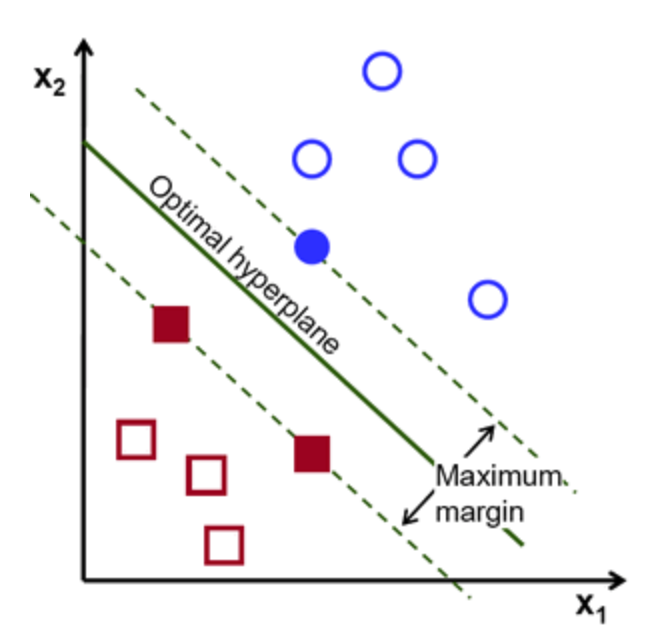
\includegraphics[width=3cm]{figs/svm.png}\\
		\end{tabular}
	}
	\caption{Otimização por SVM \cite{ref_towardsdata}}		
	\label{f.nunes}
	
\end{figure}

Já no caso de um SVM não linear, a classificação dos dados é calculada substituindo o produto escalar das proporções dos mesmo por uma função kernel\cite{ref_moro}. Segundo Moro e Aria, as SVMs podem produzir resultados de classificação precisos e robustos em uma base teórica sólida, mesmo quando os dados de entrada são não-monótonos e não-linearmente separáveis. E, embora a metodologia não forneça uma função de pontuação paramétrica, sua aproximação linear local pode oferecer um suporte importante para reconhecer os mecanismos que ligam diferentes índices à classificação final dos dados.

\pagebreak

\section{Metodologia}
\label{s.metodologia}
Toda a pesquisa foi baseada em 4 macro principais estágios de análise de dados: Extração, Estruturação, Classificação e Predição. Além disso, para detalhar tem-se 7 microestágios correspondentes.

Divide-se a pesquisa em:
\begin{enumerate}
	
	\item Extração de dados de uma origem open-source;
	
	\item Estruturação das imagens no formato PGM;
	
	\item Extração dos dados para uma planilha CSV;
	
	\item Estruturação dos dados socioecônomicos abertos;
	
	\item Concepção de classes baseados nos dados socioeconômicos;
	
	\item Predição com modelos de Machine Learning; E
	
	\item Validação dos dados.
	
\end{enumerate}

Na primeira etapa da pesquisa foi necessário um modelo para obter elementos em imagens de satélite e sócioeconômicos. A linguagem escolhida desde o início do projeto para construir o sistema foi o Python em conjunto com o R. Tal escolha baseou-se na alta demanda da mesma atualmente e na quantidade de bibliotecas que auxiliam nos estudos de Machine Learning. Foram utilizados o seguinte banco de dado imagético: National Geophysical Data Center Nighttime Lights Time Series para compor as imagens de dados de satélites noturnos. Além disso, todas as imagens foram computadas em TIF.

Para o segundo momento, foi necessário definir padronização dos formatos dos dados. Nessa etapa, foi estabelecido que seria utilizado PGM como dados de imagem. Para tanto, foram convertidas todas imagens TIFF para PGM em uma planilha csv. Na extração a intensidade luminosa dos mapas noturnos foram colocados em um arquivo CSV com 198 pixels. Nesse caso, cada imagem é convertida em uma linha com 198 colunas.

Depois disso foi necessário criar classes dos dados. Para tanto, usaram-se os índices de Produto Interno Bruto (PIB) de 2010 obtidos na pesquisa do IBGE, e foram auferidos classes utilizando KMEANs e PIB para comparar com o classificador SVM.

Por fim, utilizamos o SVM baseado em 3 classes: menor, médio e maior. Ambas se baseiam em cidades com mínimo, médio e máximo das cidades de São Paulo.

\pagebreak

\section{Apresentação e Análise de dados}
\label{s.apresentacao_analise}
No primeiro mês de projeto, foi estruturada a origem dos dados que seriam utilizados, para que pudesse assim ser definido modelo e classificação dos dados. Para tanto, todas as procuras foram guiadas em encontrar dados abertos. Na pesquisa \textit{Combining satellite imagery and machine learning to predict poverty} usada como referência para o projeto, foram utilizados dados do portal National Geophysical Data Center para predizer dados da Nigéria e Uganda. A justificativa inicial foi vinculada às facilidades e qualidades dos dados do portal, portanto, partiu-se do mesmo pressuposto no projeto. E a escolha beneficiou em automatizar o processo da obtenção grande quantidades dos dados, como podemos ver na Figura 4.

\begin{figure}[!ht]
	\centerline{
		\begin{tabular}{c}
			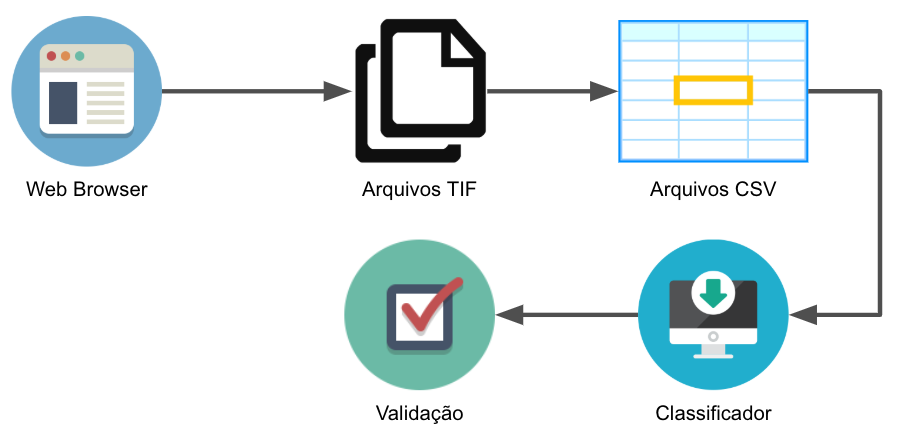
\includegraphics[width=9cm]{figs/fluxograma.png}\\
		\end{tabular}
	}
	\caption{Processos para obtenção de dados (Fonte: Autor)}		
	\label{f.nunes}
	
\end{figure}

Primeiramente, esperamos obter dados de 10  por 10 km em arquivos TIF. A escolha da quilometragem assegura que a localização obtida no mapa estivesse na análise. A contabilização realizada foi uma avaliação de um ponto como:
\begin{itemize}
	\item 10 km de longitude = 10*(360/23903.297); E
	\item 10 km latitude= 10*(360/40075.00).
\end{itemize}

Realizou-se a obtenção de 3.075 imagens realizando o download baseado nas máximas e mínimas longitudes e latitudes do estado de Estado de São Paulo. Por fim, foram obtidos dados de todos satélites, porém utilizaram-se imagens apenas do ano de 2010 os satélites. Obtidos os dados, foi escolhido convertê-los para uma análise de pixels em 198.

Depois de elencadas as imagens, foi preciso rotular os dados com as referentes cidades. Para tanto utilizamos a API do Google Maps, com ele foi possível enviar as latitutes e longitudes para obter o nome da área referente.Com isso, foi possível identificar 425 de 645 nos municípios do estado de São Paulo.

Após tal fato, foi possível escolher a maneira mais aconselhável para predizer os dados. Primeiramente, elencaram-se em duas classes para usar como dados rotulados. A primeira classe foi escolhida baseada na classificação World Bank\cite{ref_woldbank}, a qual divide como PIB:
\begin{enumerate}
	
	\item Baixo: Renda menor ou igual a U\$3955;
	
	\item Médio: Renda entre U\$3955 e U\$12235; E
	
	\item Alto: Maior ou igual a U\$12235.
	
\end{enumerate}

Com essa classificação foram obtidos os seguintes dados:

\begin{figure}[!ht]
	\centerline{
		\begin{tabular}{c}
			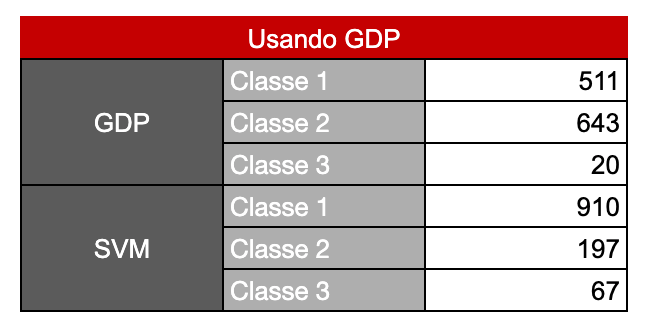
\includegraphics[width=5cm]{figs/gdp_results.png}\\
		\end{tabular}
	}
	\caption{Desempenho por classes utilizando KMeans (Fonte: Autor)}		
	\label{f.nunes}
	
\end{figure}

Na segunda classe procurou-se rotular os dados otimizando com um classificador. Kmeans trouxe as seguintes classes para análise:

Com os dados rotulados, utilizou-se o SVM para classificar as imagens auferidas. Essas 3 classes baseadas na quantidade de pixels, estabelecemos 3 cidades que seriam usadas como base para o classificador. Do mais baixo para o maior tivemos:

\begin{itemize}
	\item Menor = Lucianópolis com uma soma de 0 pixels;
	\item Médio = Pirangi com 4558.0 pixels; E
	\item Alto = São Paulo com a soma de 114735.0 pixels.
\end{itemize}

O resultado dessa classificação foi conferido em conjunto com os outros dados rotulados. Por final, foi possível o resultado de 71,47\% utilizando KMEANs e 49,83\% utilizando os classificadores da ONU.

\begin{figure}[!ht]
	\centerline{
		\begin{tabular}{c}
			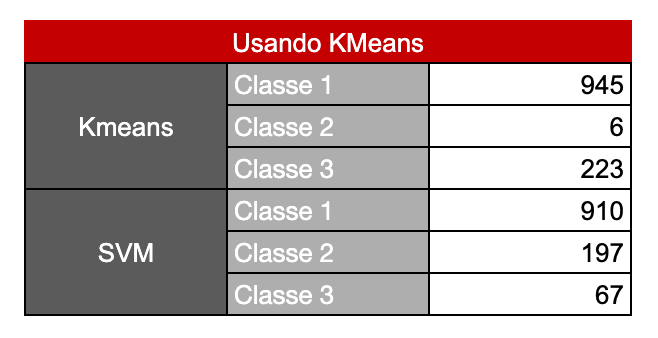
\includegraphics[width=5cm]{figs/kmeans_results.png}\\
		\end{tabular}
	}
	\caption{Desempenho por classes utilizando GDP (Fonte: Autor)}		
	\label{f.nunes}
	
\end{figure}

Outro bom indicador é analisar as 3 imagens com os classficadores pelo mapa do estado de São Paulo.

\begin{figure}[!ht]
	\centerline{
		\begin{tabular}{c}
			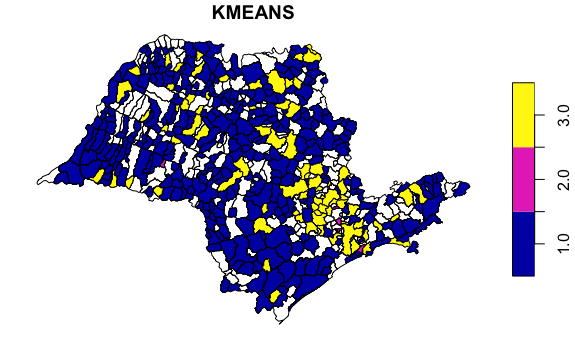
\includegraphics[width=8cm]{figs/kmeans_cities.png}\\
		\end{tabular}
	}
	\caption{Classes utilizando Kmeans (Fonte: Autor)}		
	\label{f.nunes}
	
\end{figure}

\begin{figure}[!ht]
	\centerline{
		\begin{tabular}{c}
			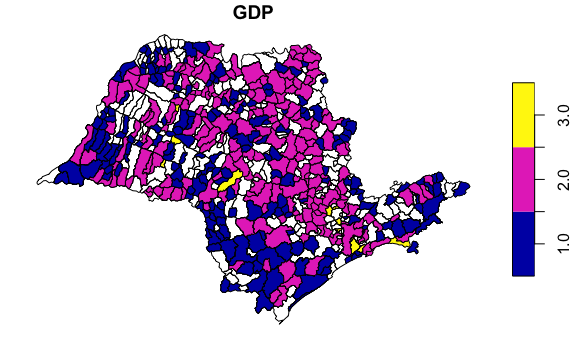
\includegraphics[width=8cm]{figs/gdp_cities.png}\\
		\end{tabular}
	}
	\caption{Classes utilizando PIB (Fonte: Autor)}		

	
\end{figure}

\begin{figure}[!ht]
	\centerline{
		\begin{tabular}{c}
			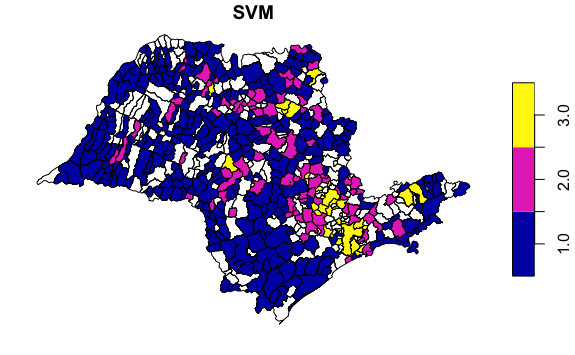
\includegraphics[width=8cm]{figs/svm_cities.png}\\
		\end{tabular}
	}
	\caption{Classes utilizando SVM (Fonte: Autor)}		
	
	
\end{figure}

\pagebreak

\section{Cronograma}
\label{s.cronograma}
O projeto foi realizado seguindo as etapas a seguir na figura \ref{f.cronograma}.

\begin{figure}[!ht]
	\centerline{
		\begin{tabular}{c}
			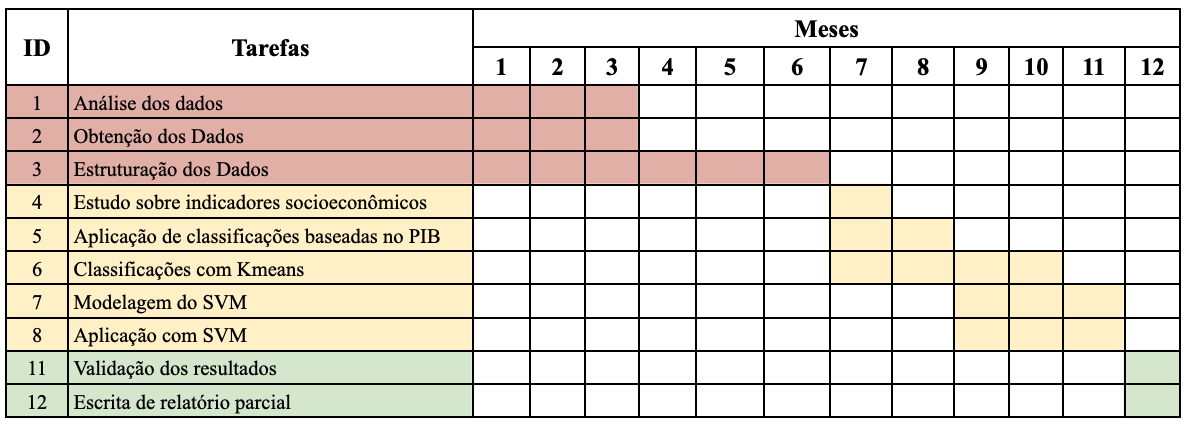
\includegraphics[width=12cm]{figs/cronograma.png}\\
		\end{tabular}
		}
		
		
		
		\caption{Cronograma de atividades da presente proposta (Fonte: Autor)}		
		\label{f.cronograma}
	
\end{figure}

\pagebreak


\section{Conclusões}
\label{s.conclusoes}
No final deste período de pesquisa, considerando a quantidade de dados obtidos, os modelos aplicados e a acurácia auferida, avalia-se com um bom resultado da mesma.

Primeiramente, foram utilizados cerca de 3.075 itens de 10 km x 10 km no formato PGMs, algo que compactua com cerca de 425 cidades do estado de São Paulo, correspondendo 65,89\% de todas. Já em um segundo momento, estruturaram-se os dados de maneira automatizada assim possibilitando utilizar dois classificadores de dados e utilizar ao menos um método de predição. Por fim, alcançando os resultados retradados na figura a seguir.

\begin{figure}[!ht]
	\centerline{
		\begin{tabular}{c}
			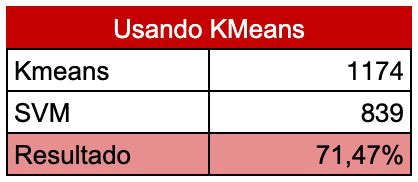
\includegraphics[width=5cm]{figs/svm_final.png}\\
		\end{tabular}
	}
	
	
	
	\caption{Resultados obtidos na pesquisa (Fonte: Autor)}		
	\label{f.cronograma}
	
\end{figure}


Porém, pode-se dizer que a pesquisa possui alguns pontos de melhora. Primeiramente, na utilização mais teórica dos dados de base, trazendo conhecimentos socioeconômicos mais refinados para então usar outros índices de desempenho econômico que iriam além do PIB.

Além disso, seria muito importante utilizar mais de uma método de Machine Learning para validar os resultados esperados. Pensa-se em continuar com os estudos para implementação da Classificação supervisionada de padrões utilizando Floresta de Caminhos Ótimos\cite{ref_floresta}, por exemplo, que provou-se ser aconselhável para uso de dados como PGM.


%----------------------------------------------------------------------------
% Bibliography

\pagebreak

\bibliographystyle{./IEEEtran}
\bibliography{refs}



%----------------------------------------------------------------------------

\end{document}
